%-----------------------------------------------------------------------------------%
\section{The Detector}\label{sec:THE_hawc}
%-----------------------------------------------------------------------------------%

\begin{figure}[h!]
    \centering{
    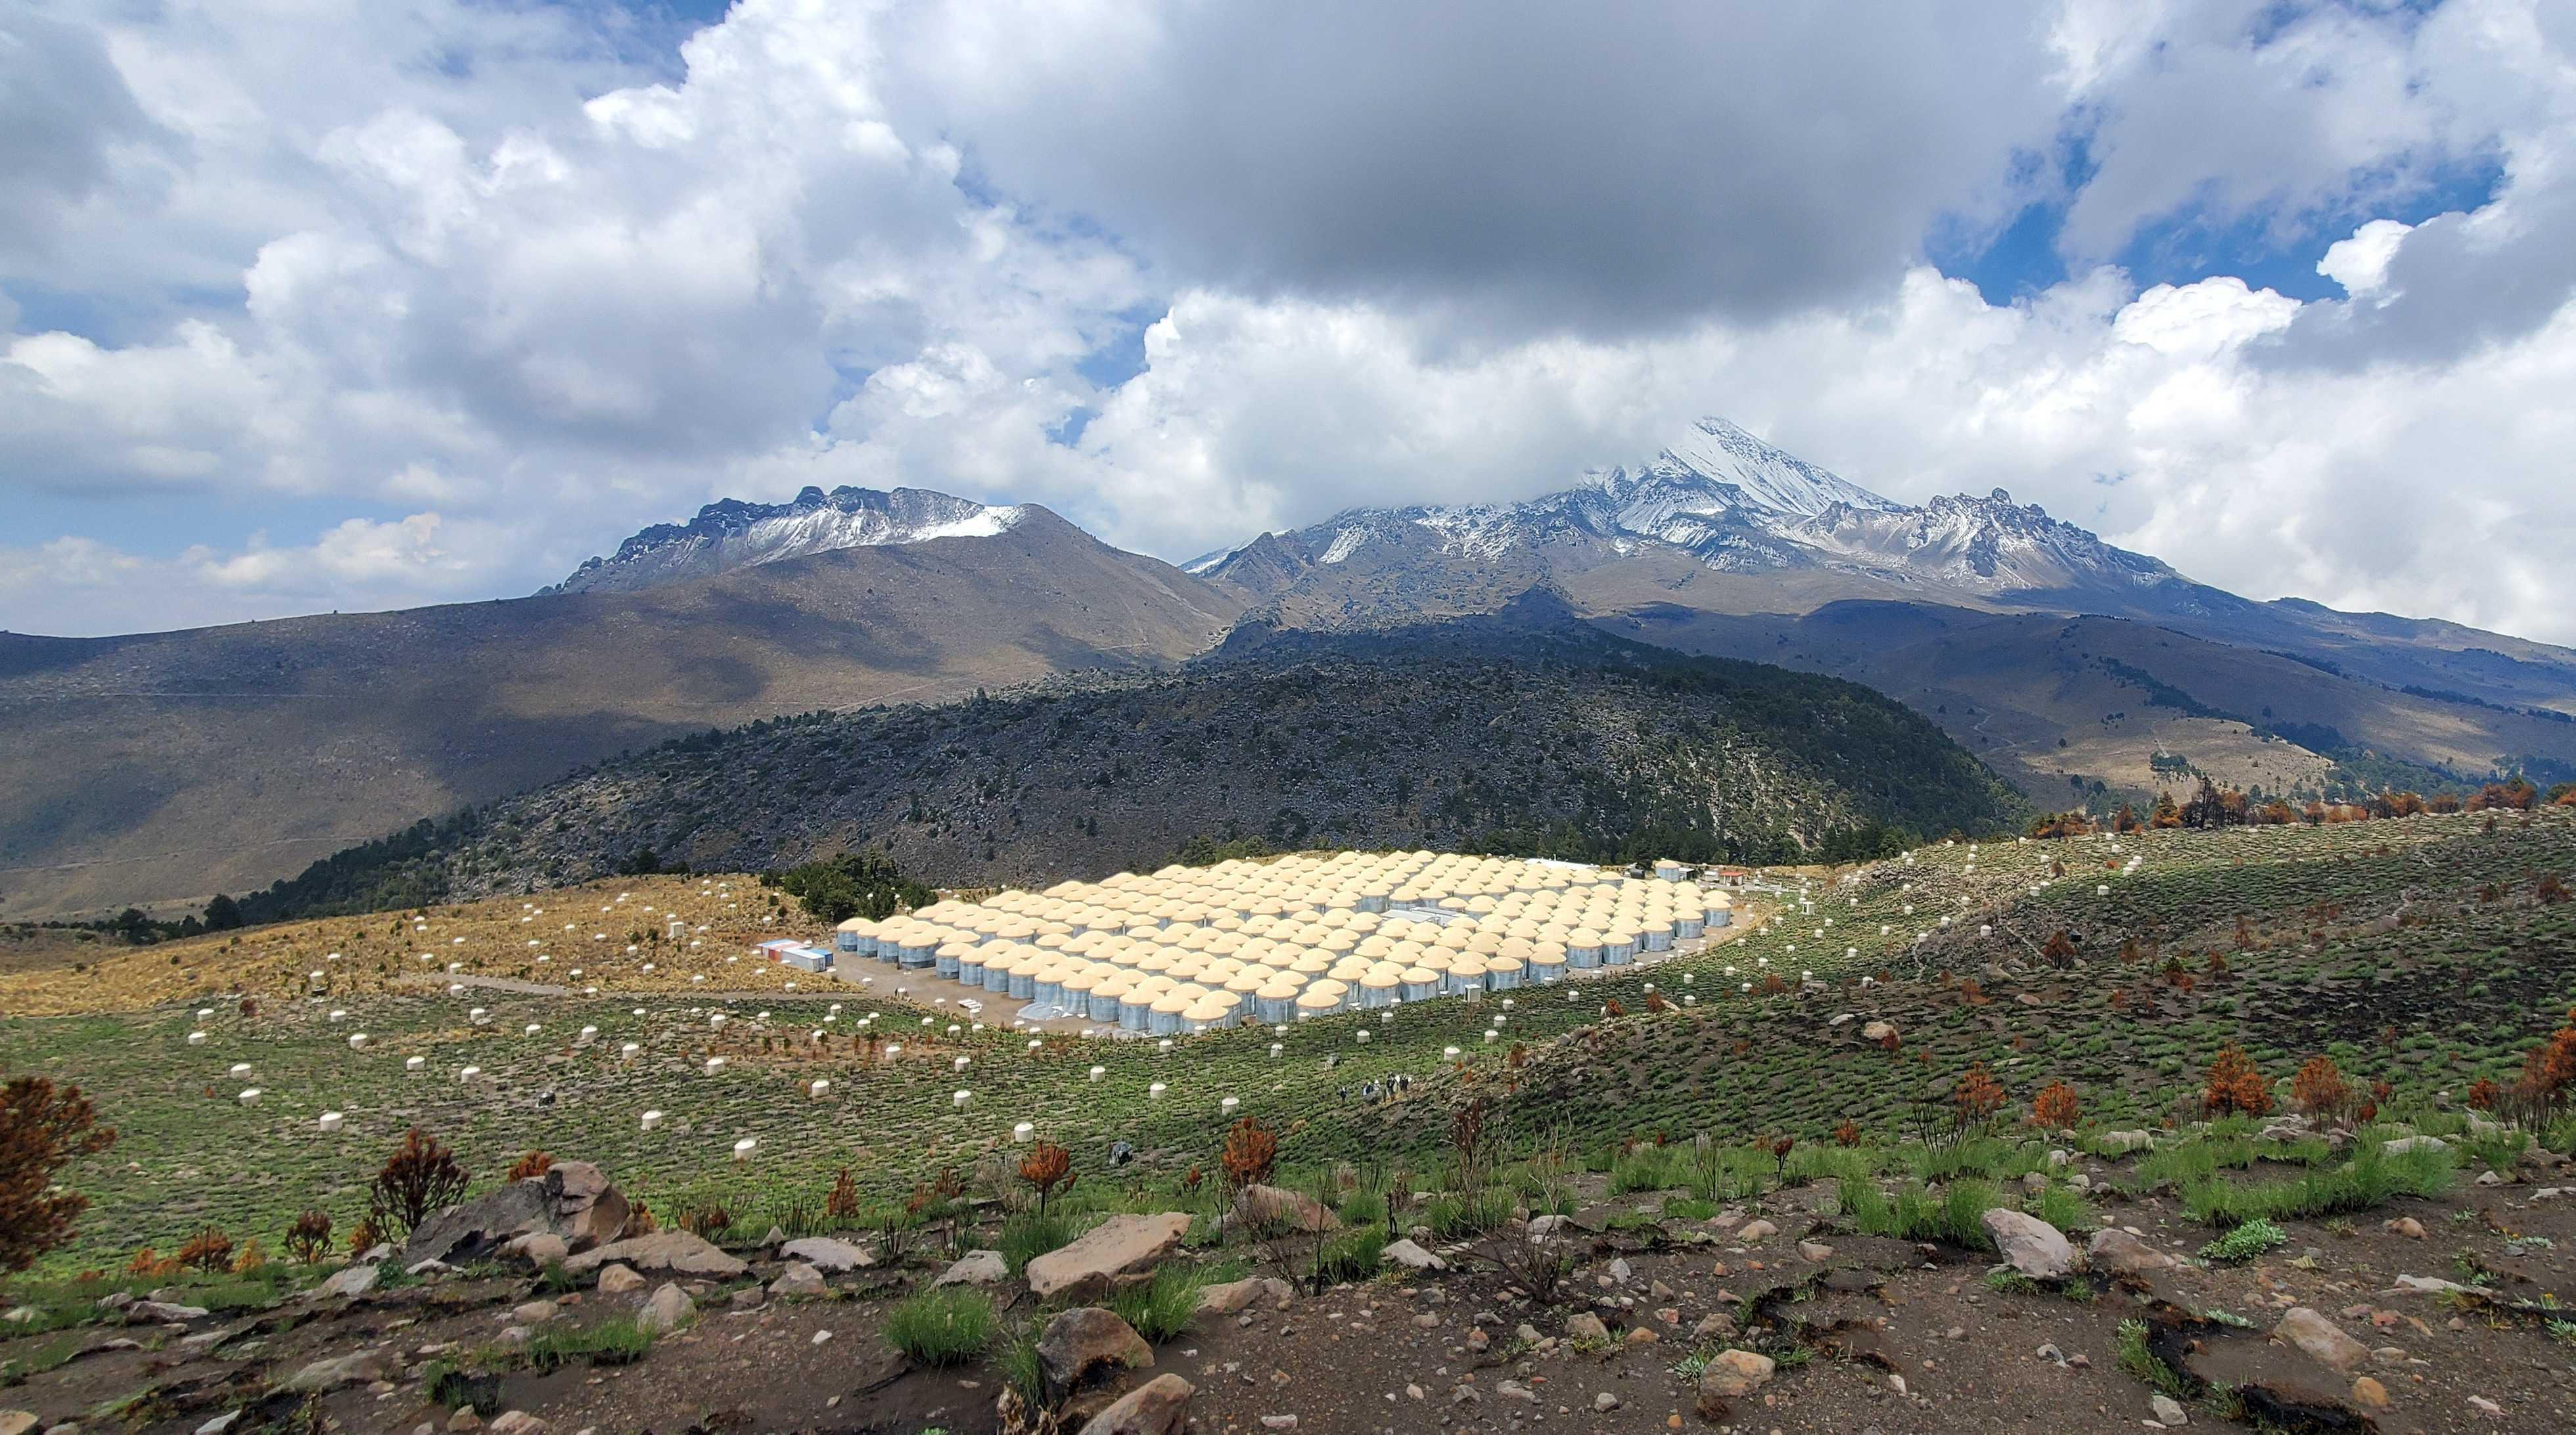
\includegraphics[scale=0.155]{figures/hawc/HAWC.jpg}
    }
    \caption{Photo of the HAWC detector that I took on May 17, 2023. Main array is centered in the photo and comprised of the larger tanks. Outriggers are the smaller tanks around the main array.}
    \label{fig:HAWC}
\end{figure}

The High Altitude Water Cherenkov (HAWC) Observatory is a specialized instrument designed for the observation of high energy gamma-rays and cosmic rays \cite{HAWC_NIM}.
Located on the Sierra Negra volcano in Mexico, HAWC observes gamma rays and cosmic rays in the energy range of approximately 100 GeV to 100's of TeV.
At an elevation of 4,100 meters, it monitors about two-thirds of the sky every day with an uptime above 90\%.
This capability is essential for studying high-energy astrophysical phenomena.

HAWC consists of 300 water Cherenkov detectors (WCDs) spread over 22,000 $m^2$.
Each main array detector is filled with purified water and equipped with four, upward-facing photomultiplier tubes (PMTs).
See \cref{fig:WCD_schematic} for a schematic of WCDs.
These PMTs detect Cherenkov radiation from charged particles passing through the tanks.
These charged particles are generated when a high energy gamma or cosmic ray collides with gas in the atmosphere to create a charged particle shower, as shown in \cref{fig:airshowers}.
Cherenkov radiation occurs when a charged particle traverse a medium faster than the speed of light withing the medium.
An electromagnetic shockwave is formed, akin to an optic boom, that corresponds with the velocity of the particle, see \cref{fig:Cherenkov_front}.

\begin{figure}
    \centering{
        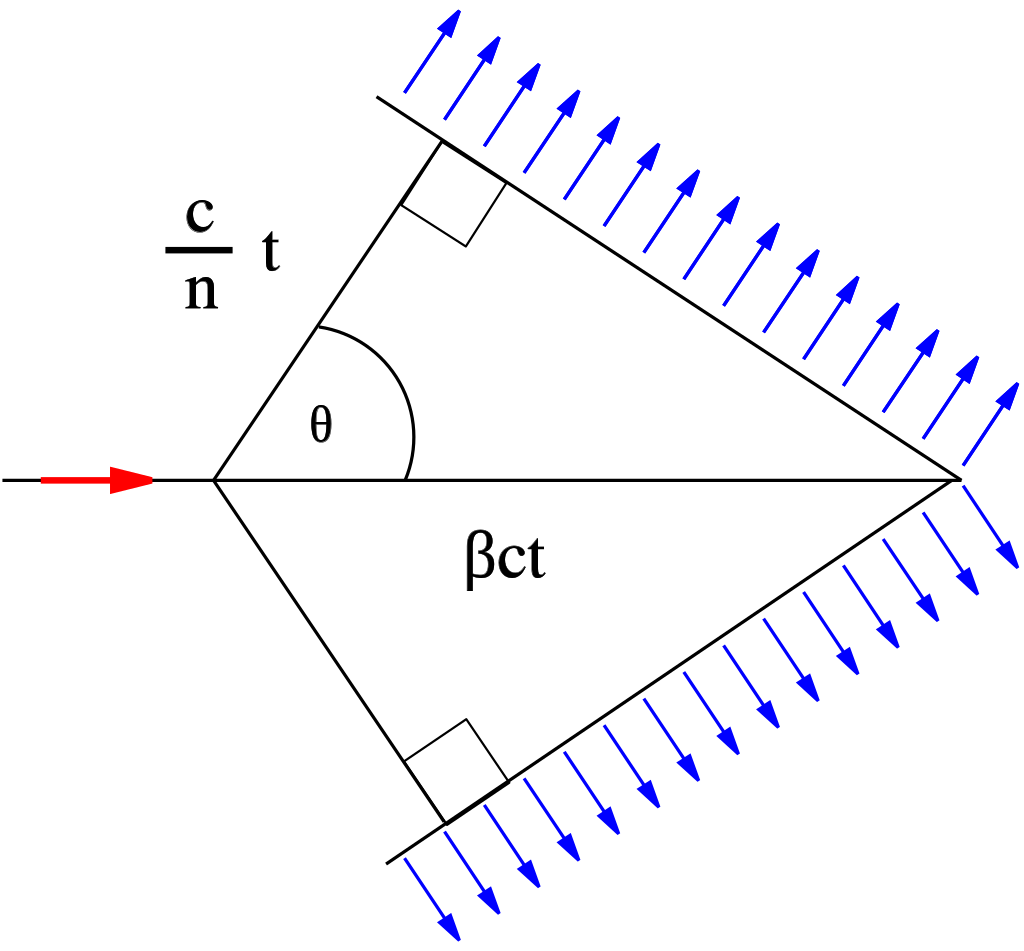
\includegraphics[scale=0.2]{figures/Cherenkov.svg.png}
    }
    \caption{Geometry of Cherenkov radiation. This occurs when a charged particle traverses a medium faster than the speed of light within the medium. The particle, red arrow, when traversing through water, will create an optical shockwave that emits blue light. The angle of the Cherenkov cone will depend on the speed of the particle ($\beta c$) and the index of refraction ($n$) in the media. Figure from \cite{Cherenkov_front}.}
    \label{fig:Cherenkov_front}
\end{figure}

The observatory includes a separate tank configuration which are referred to as the outriggers.
They are a secondary array of 345 smaller WCD's.
Surrounding the main array, each outrigger tank measures 1.55 meters in diameter and height and contain a single upward-facing 8-inch PMT.
This add-on increases the instrumented footprint fourfold.
The outriggers are meant to improve the reconstruction of showers extending beyond the main array, especially for events above 10 TeV.
However, at the time of writing this thesis, the outriggers have not been fully integrated into HAWC's reconstruction software.

\begin{figure}
    \centering{
    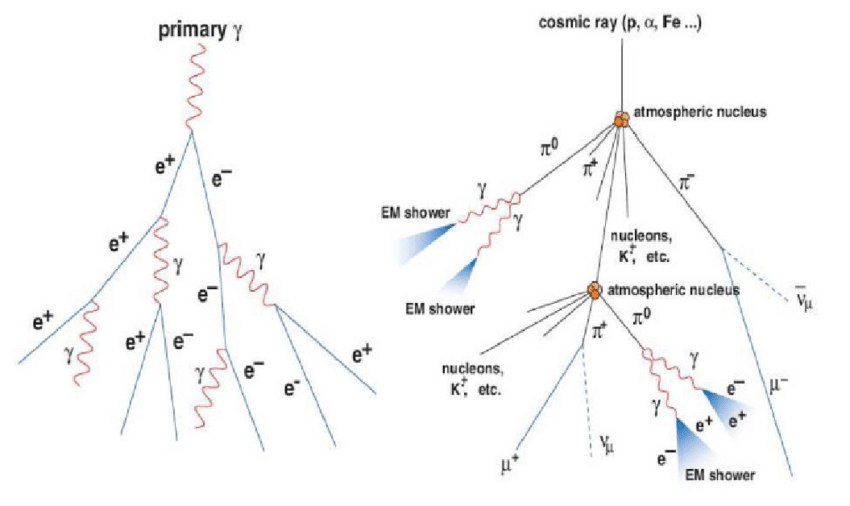
\includegraphics[scale=0.5]{figures/hawc/high_energy_air_shower.png}
    }
    \caption{A particle physics illustration of high energy particle showers. Left shower is an electromagnetic shower from a high energy gamma-ray. Most particles in the shower will be a combination of photons and charged leptons, in this case electrons and positrons ($e^\pm$). Right figure shows a cosmic ray particle shower. The cosmic ray will produce many more types of particles including pions ($\pi$), neutrinos ($\nu$), and other charged leptons. Figured pulled from \cite{lopez_thesis}.}
    \label{fig:airshowers}
\end{figure}

%-----------------------------------------------------------------------------------%
\subsection{Construction and Hardware} \label{sec:hawc_hardware}
%-----------------------------------------------------------------------------------%

\begin{figure}
    \centering{
        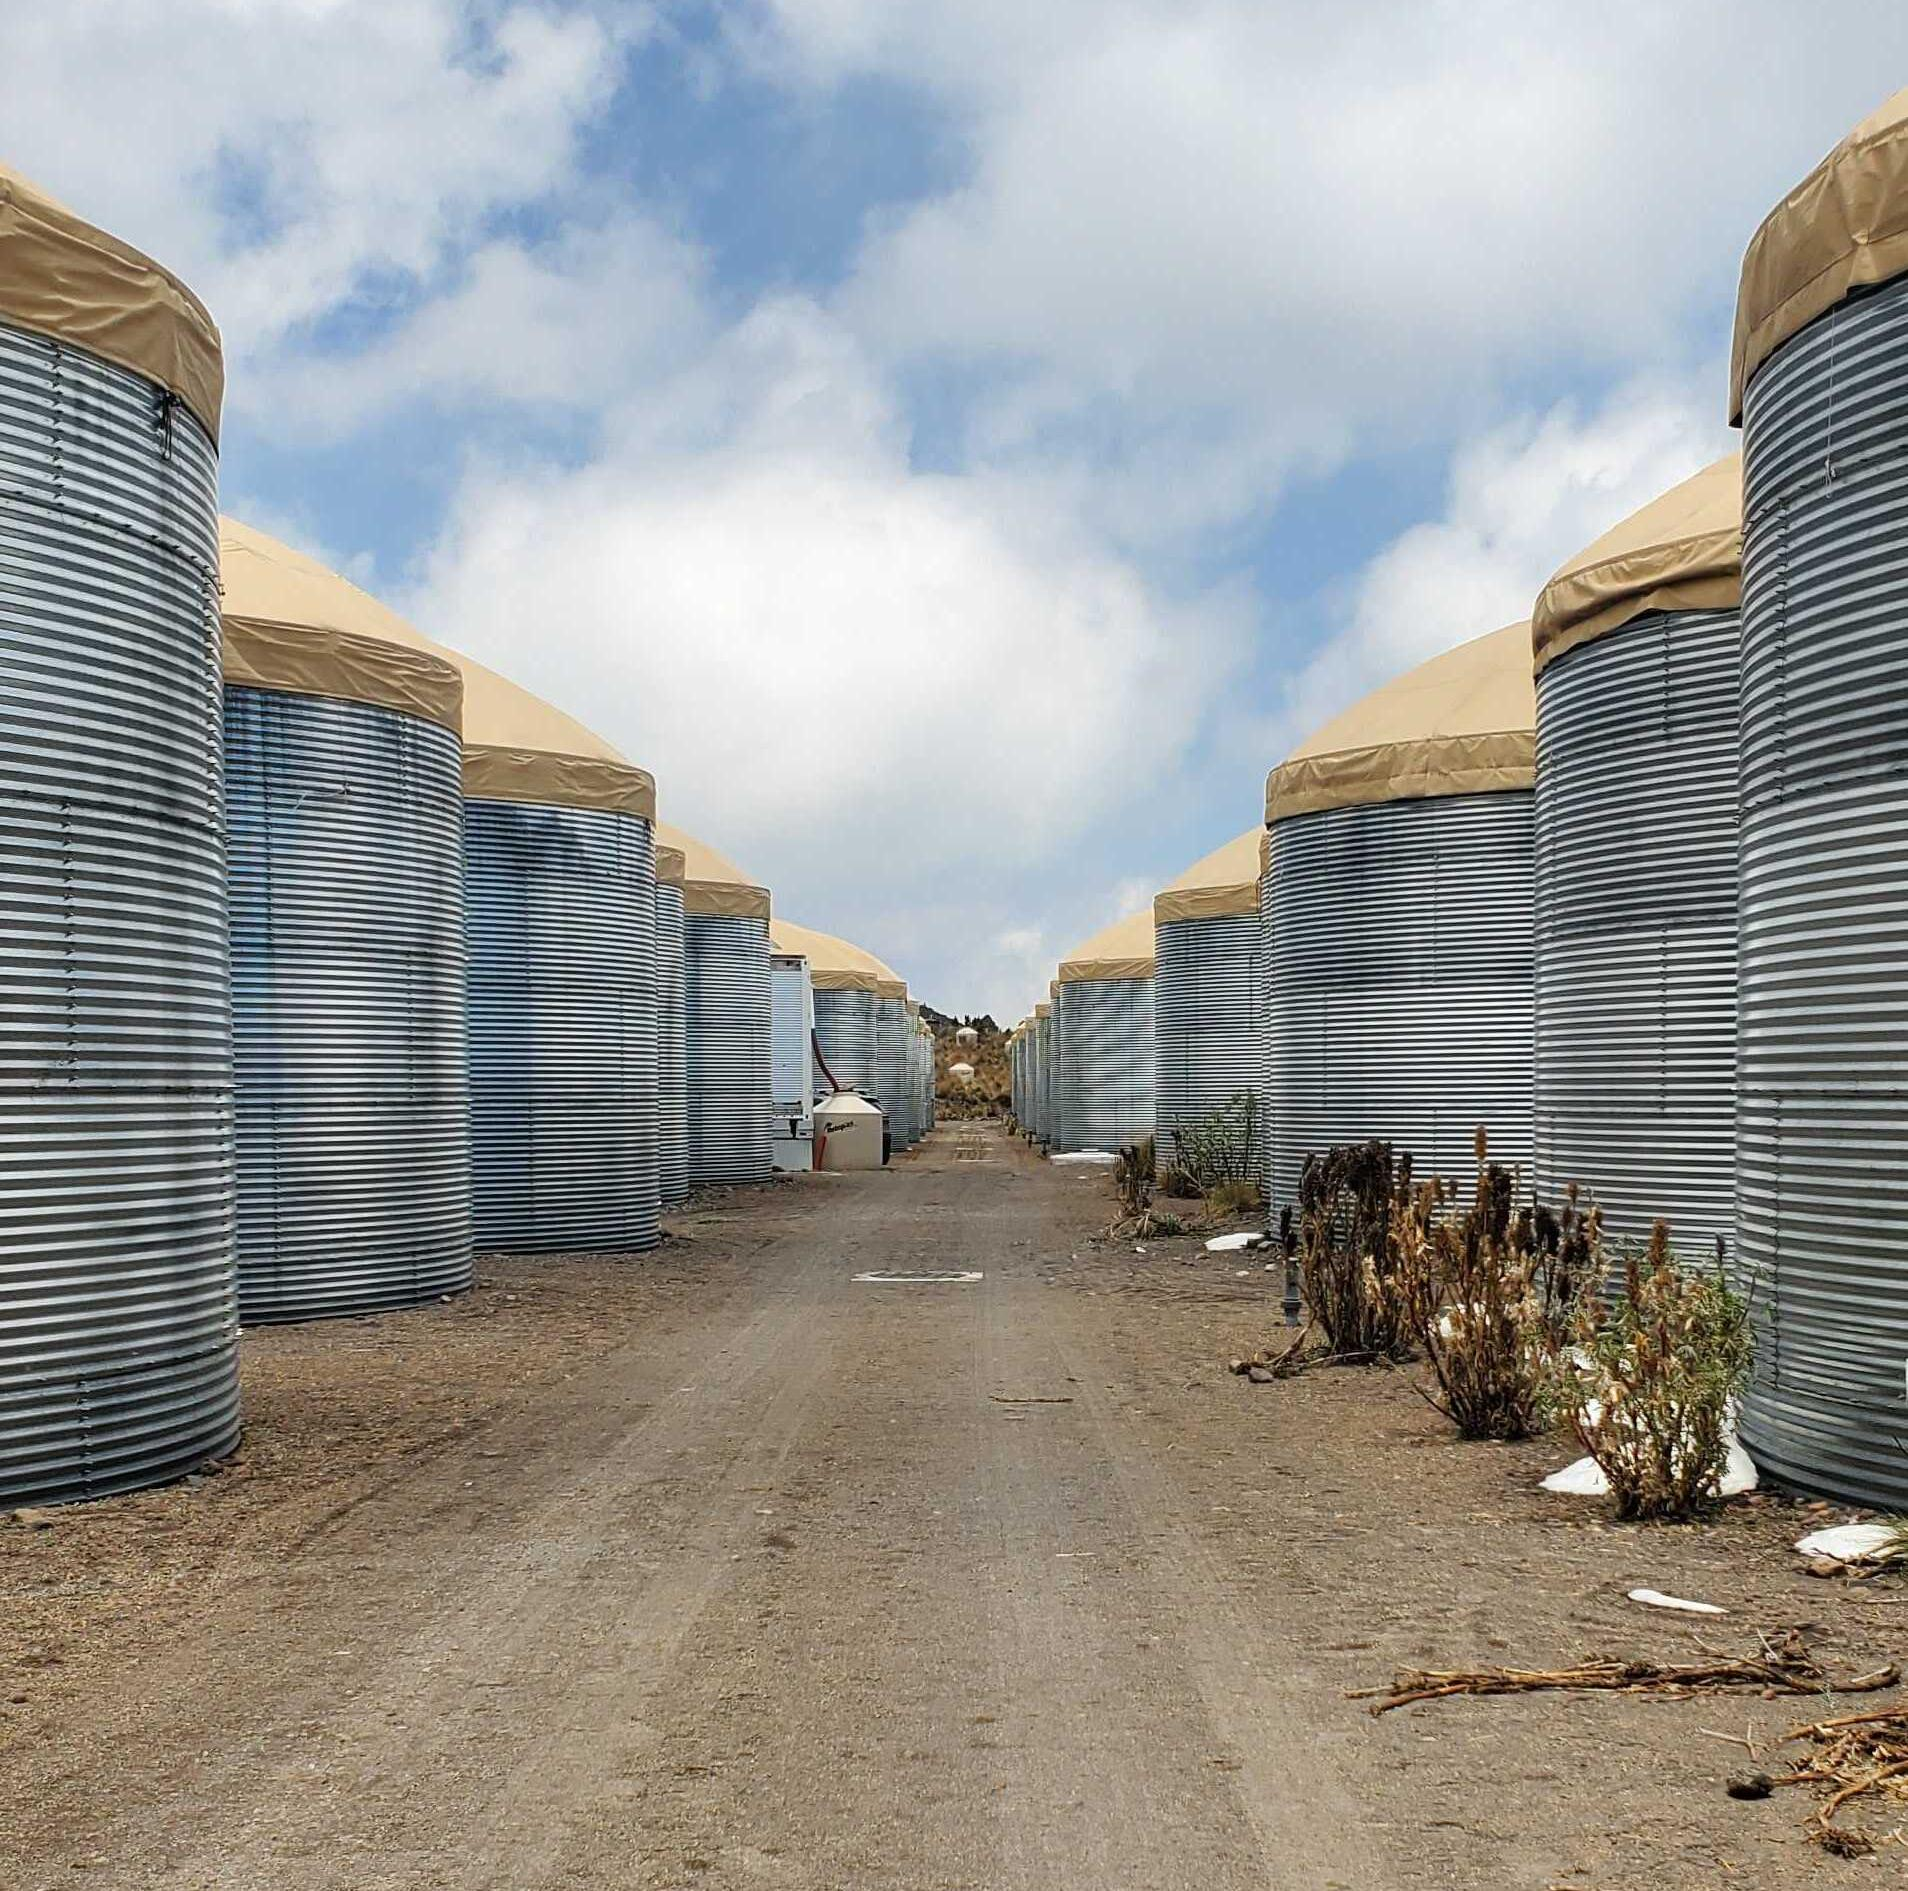
\includegraphics[scale=0.14]{figures/hawc/WCDs.jpg}
        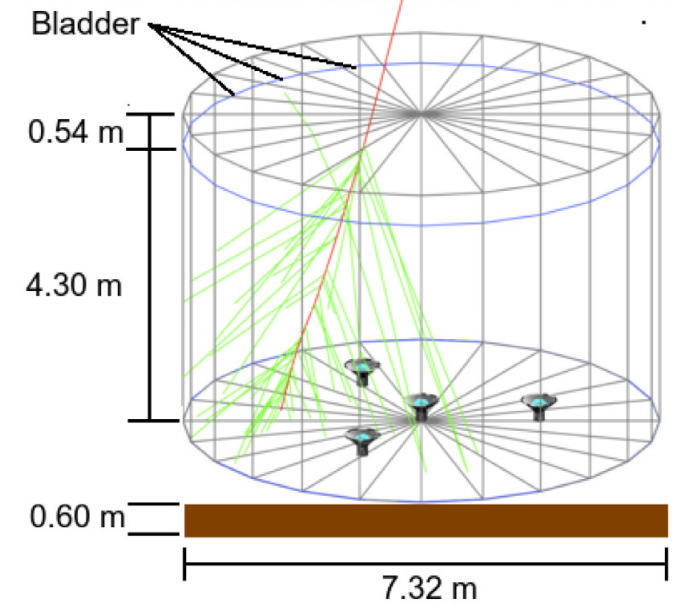
\includegraphics[scale=0.45]{figures/hawc/WCD_schematic.png}
    }
    \caption{The WCDs. Left image features several WCDs looking from within the main array of HAWC. Right image shows a schematic of a WCD pulled from \cite{HAWC_NIM}.}
    \label{fig:WCD_schematic}
\end{figure}

Each main array WCD, see \cref{fig:WCD_schematic}, is a cylindrical tank with dimensions of 7.3 m in diameter and 5.4 m in height and filled with 180,000 L of water \cite{HAWC_NIM}.
The metal shell of these tanks is made from corrugated, galvanized steel panels bolted together.
The interior of each tank is lined with a black, low-density polyethylene bladder, designed to be impermeable to external light and to prevent reflection of Cherenkov light within the tank.
This bladder is approximately 0.4 mm thick of low-density polyethylene.
To further minimize light penetration, a black agricultural foil covers the bladder.
The ground and walls inside the tank are protected with felt and sand to safeguard against punctures.
The tanks are filled 4.5 m deep of purified water, achieving a photon attenuation length for Cherenkov photons that exceeds the tank's dimensions \cite{HAWC_NIM}.
This purification level ensures the optimal detection environment for the photons generated by traversing charged particles.

At the base of each tank, four photomultiplier tubes (PMTs) are installed to detect the Cherenkov radiation emitted by charged particles in water.
Three 8-inch diameter PMTs surround a larger 10-inch PMT from Hamamatsu \cite{hawc_pmt}.
The variation in PMT response is carefully accounted for in event reconstruction algorithms.
Signals from the PMTs traverse 610 ft cables to the counting house, where they are processed by Front-End Boards (FEBs), see \cref{fig:basic_tanks_schem,fig:dig_schem}.
These FEBs, along with Time to Digital Converters (TDCs), digitize the signals and manage the high voltage supply to the PMTs.

%-----------------------------------------------------------------------------------%
\subsection{Data Acquisition and Signal Processing} \label{sec:hawc_daq}
%-----------------------------------------------------------------------------------%

\begin{figure}
    \centering{
        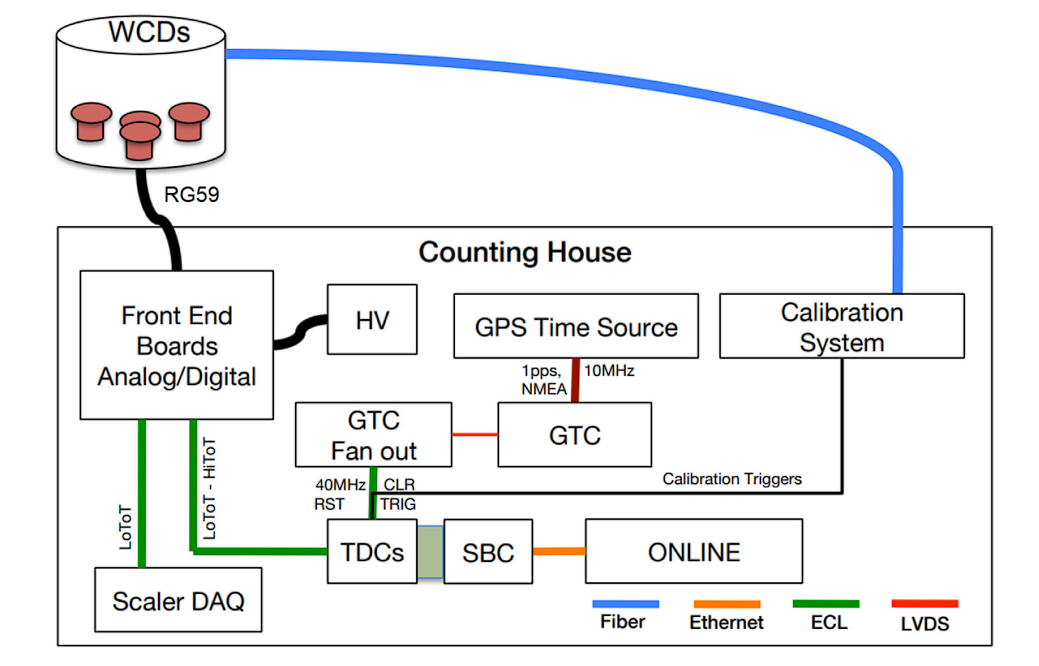
\includegraphics[scale=0.5]{figures/hawc/tank_basic_schem.png}
    }
    \caption{Overview of HAWC control and data electronics. The LoToT and HiToT threshold signals are discussed in \cref{sec:hawc_daq}. Figure from \cite{HAWC_NIM}}
    \label{fig:basic_tanks_schem}
\end{figure}

\begin{figure}
    \centering{
        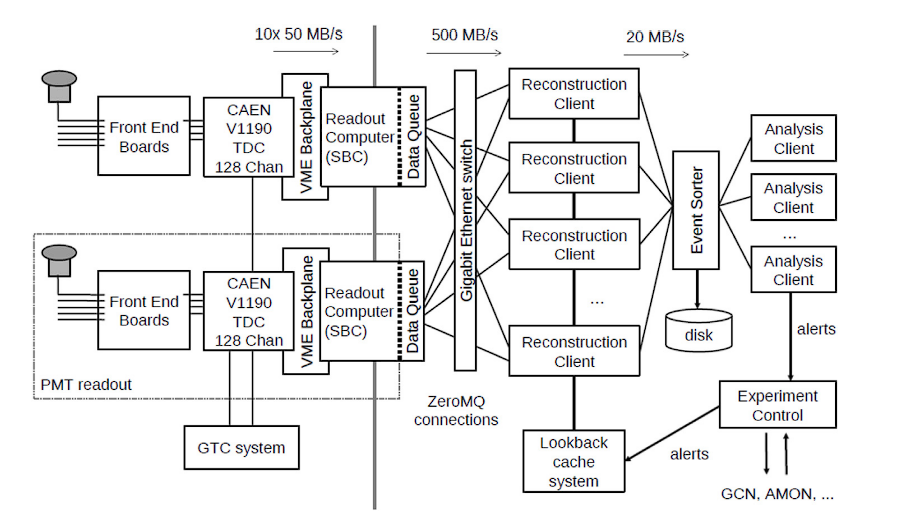
\includegraphics[scale=0.6]{figures/hawc/digital_schematic.png}
    }
    \caption{Schematic of data flow in HAWC data acquisition and online processing system. Pulled from \cite{HAWC_DAQ_NIM}.}
    \label{fig:dig_schem}
\end{figure}

The HAWC data acquisition (DAQ) and signal processing systems convert the physical detection of particles into analyzable data.
This process involves a series of steps from initial signal detection by PMTs to digital conversion and preliminary analysis, see \cref{fig:dig_schem,fig:tot_threholds}.

\begin{figure}
    \centering{
        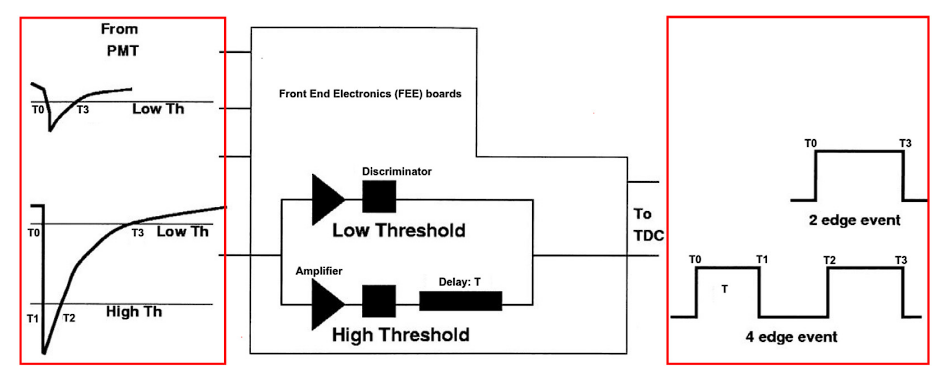
\includegraphics[scale=0.6]{figures/hawc/ToT_threshold.png}
    }
    \caption{How HAWC FEB initially processes analog PMT signals. Signals are split through an amplifier and discriminator circuit. Each path is designated for either the HIGH or LOW threshold for the signal. The 2-edge event corresponds to LOW, while the 4 edge corresponds to HIGH. Figure from \cite{HAWC_DAQ_NIM}.}
    \label{fig:tot_threholds}
\end{figure}

Once the signal from the PMTs arrive at the counting house, they enter the Front-End Boards (FEBs).
The FEBs are responsible for the initial processing of these signals, which includes amplification and integration \cite{Milagro_DAQ}.
Each PMT signal is compared against preset LOW/HIGH voltage thresholds in the FEBs, see \cref{fig:tot_threholds}, identifying signals that correspond to about 1/4 and 4 photoelectrons, respectively.
This differentiation allows the system to gauge the strength of the detected Cherenkov radiation.
The processed signals are then digitized by Time to Digital Converters (TDCs).
These converters measure the time over threshold (ToT) for each signal, a parameter that reflects both the duration and amplitude of the signal.
This digitization facilitates reconstruction of the original event for translating the physical interactions within the detectors into data \cite{HAWC_NIM,HAWC_DAQ_NIM,Milagro_DAQ}.

Synchronization across the HAWC observatory is maintained by a central GPS Timing and Control (GTC) system, which achieves a timing resolution of 98 ps.
This high-resolution timing is vital for accurately reconstructing the timing and location of air showers initiated by cosmic and gamma rays.
The GTC system ensures that all components of the DAQ operate in unison to preserve the temporal integrity of the detected events \cite{HAWC_NIM,hawc_daq_thesis}.

Once digitized, the data are transferred to an online event reconstruction system.
This system runs the Reconstruction Client, which utilizes the raw PMT data to reconstruct the characteristics of the air showers, such as their direction and energy \cite{HAWC_DAQ_NIM}.
The capacity for real-time analysis allows HAWC to promptly respond to astrophysical phenomena like Gamma Ray Bursts (GRBs) and to participate in multi-messenger astronomy by following up on alerts from other observatories.
This real-time processing system is designed to handle high data throughput, using ZeroMQ \cite{zeromq} for efficient data transfer between software components.
Analysis Clients perform specific online analyses that require immediate data, including monitoring for GRBs, solar flare activity, and participation in global efforts to track gravitational waves and neutrinos \cite{HAWC_NIM}.

The DAQ system is overseen by an Experiment Control system and crew that manage the operational aspects of data collection.
This includes initiating and terminating data collection runs and monitoring the experiment for errors.
In the event of a system crash, often caused by environmental factors such as lightning, the Experiment Control system is designed to automatically restart the experiment and minimize downtime \cite{HAWC_NIM,HAWC_DAQ_NIM}.

%-----------------------------------------------------------------------------------%
\section{Event Reconstruction} \label{sec:hawc_reconstruction}
%-----------------------------------------------------------------------------------%

Event reconstruction at the HAWC Observatory is a critical procedure that converts the raw data from the observatory's WCDs into a coherent framework for understanding cosmic and gamma-ray events.
This process includes several distinct steps.
Core Fitting determines the geometric center of the air shower on the detector plane.
Angle Reconstruction assesses the trajectory of the incoming particle, revealing its origin in the sky.
Energy Estimation is performed using both \textit{f}-hit and Neural Network (NN) methods to quantify the energy of the detected events.
Gamma/Hadron discrimination differentiates between gamma-ray and hadronic cosmic ray initiated showers, a vital step for astrophysical interpretations.
Each of these steps is described in more details in the following sections.

%$$$$$$$$$$$$$$$$$$$$$$$$$$$$$$$$$$$$$$$$$$$$$$$$$$$$$$$$$$$$$$$$$$$$$$$$$$$$$$$$$$$%
\subsection{Core Fitting} \label{sec:hawc_core_fitting}
%$$$$$$$$$$$$$$$$$$$$$$$$$$$$$$$$$$$$$$$$$$$$$$$$$$$$$$$$$$$$$$$$$$$$$$$$$$$$$$$$$$$%

\begin{figure}[h!]
    \centering{
    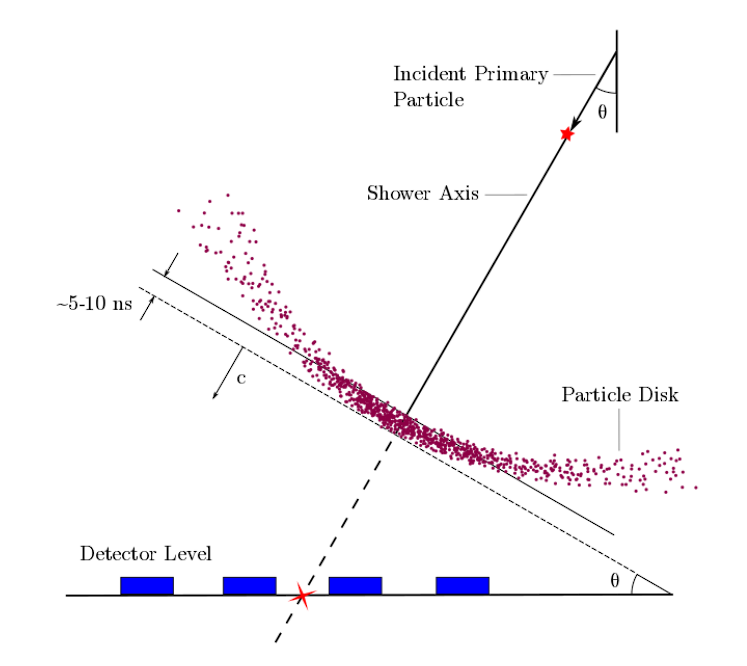
\includegraphics[scale=0.5]{figures/hawc/shower_shape.png}
    }
    \caption{A particle shower incident on WCDs. Secondary particles of an air shower travel in a cone centered on primary incident particle. Reconstruction of the initial angle is possible with arrival time of hits in PMTs inside WCDs. Figure from \cite{thesis_Zigg}.}
    \label{fig:shower_shape}
\end{figure}

In the study of air showers, accurately determining the location of the air shower core on the ground is crucial for reconstructing the direction of the originating primary particle.
An illustration of this can be seen in a HAWC event plot, \cref{fig:shower_shape,fig:ldf_particleshower}, where the lateral charge distribution across the array is displayed.
The core is identified and marked with a red star in \cref{fig:shower_shape}, reconstructed using a predetermined functional form, \cref{eq:hawc_showercore}.
We model the signal, $S_i$, from the \textit{i}th PMT by following the equation
\showercore
In this model, $\tilde{x}$ represents the core location and $\tilde{x}_i$ is the position of the \textit{i}th PMT.
$R_m$ stands for the Molière radius, which is approximately 120 meters at the altitude of HAWC.
$\sigma$ is the standard deviation of the Gaussian distribution.
$N$ is the normalization factor for the tail of the distribution.
The equation incorporates fixed values of $\sigma = 10$ m and $N=5.10^{-5}$.
This leaves the core location and overall amplitude $A$ as the free parameters to be determined during fitting.

\begin{figure}
    \centering{
        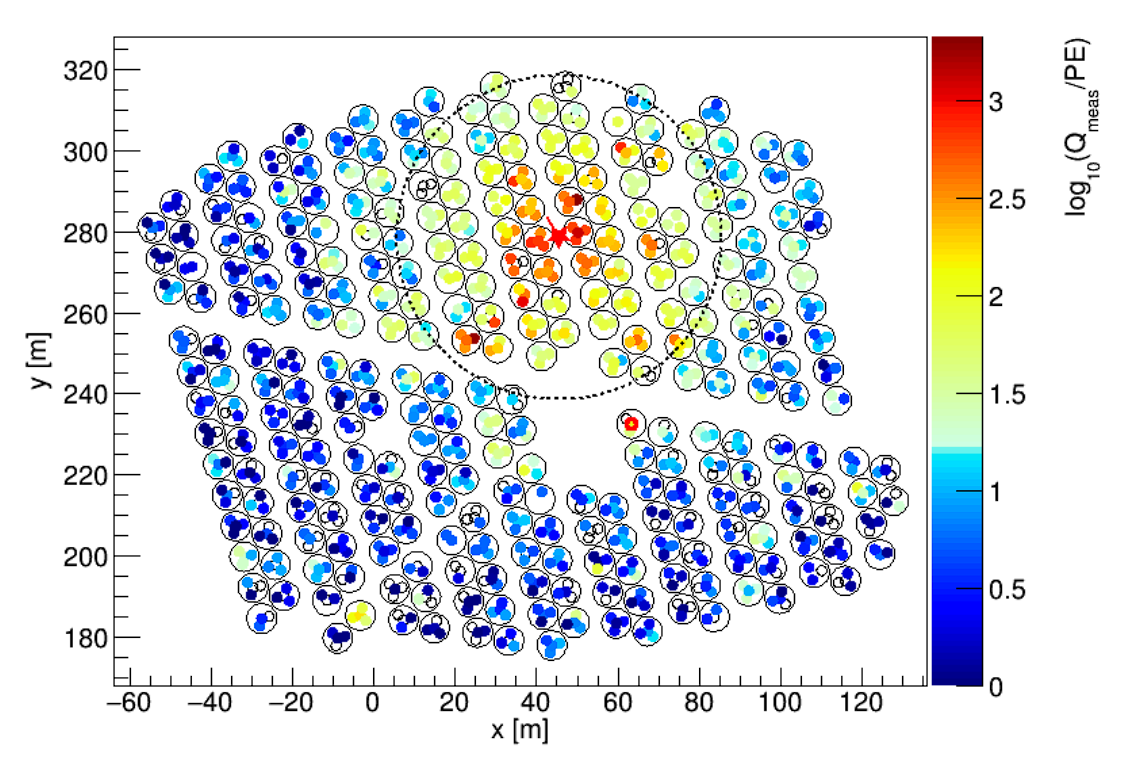
\includegraphics[scale=0.5]{figures/hawc/core_fitting.png}
    }
    \caption{Charge deposition in each PMT for a reconstructed gamma-ray event. WCDs are outlined in black surrounding the 4 smaller circles that represent PMTs. The color scale indicates the charge deposition in each PMT. The best shower core fit from Super Fast Core Fit (SFCF) is noted with a red star in the center of the dashed circle \cite{Abeysekara_2017}.}
    \label{fig:core_fitter}
\end{figure}

The chosen functional form for the Super Fast Core Fit (SFCF) algorithm is a simplified version of a modified Nishimura-Kamata-Greisen (NKG) function \cite{cosmic_ray_shape}, selected for its computational efficiency which is essential for rapid fitting of air shower cores.
The SFCF form allows numerical minimization to converge more quickly due to the function's simplicity, the analytical computation of its derivatives, and the absence of a pole at the core location \cite{Abeysekara_2017}.
\Cref{fig:core_fitter} provides a visualization of a recorded event, with the plot depicting the charge recorded by each PMT as a function of the distance to the reconstructed shower core.
Through the application of the SFCF, core locations can be identified with a median error of approximately 2 m for large events and about 4 m for smaller ones, assuming the gamma-ray event core impacts directly upon the HAWC detector array \cite{Abeysekara_2017}.
It is noted that as the core's distance from the main array increases, the precision in locating the core diminishes \cite{Abeysekara_2017}, highlighting the importance of proximity in the accuracy of core reconstruction.


%$$$$$$$$$$$$$$$$$$$$$$$$$$$$$$$$$$$$$$$$$$$$$$$$$$$$$$$$$$$$$$$$$$$$$$$$$$$$$$$$$$$%
\subsection{Angle Reconstruction} \label{sec:hawc_angleReco}
%$$$$$$$$$$$$$$$$$$$$$$$$$$$$$$$$$$$$$$$$$$$$$$$$$$$$$$$$$$$$$$$$$$$$$$$$$$$$$$$$$$$%

After establishing the core position, the next step is angle reconstruction.
This process determines the primary particle's trajectory.
The angle of arrival is indicative of the originating gamma ray's direction.
It correlates to the cosmic source of the gamma-ray.
We deduce this angle using the timing of PMT hits \cite{Abeysekara_2017}.

The air shower's front is conically shaped, not flat.
This shape arises from the travel patterns of secondary particles.
An event example is illustrated in \cref{fig:shower_shape}.
Far from the core, secondary particles undergo multiple scattering.
They also travel longer distances \cite{wcd_Sensitivity}.
Particle sampling decreases with distance from the core.
This decrease results in measurable delays in arrival times \cite{wcd_Sensitivity,Abeysekara_2017}.
Simulations provide a corrective measure for these effects.
The correction is a function of shower parameters \cite{Abeysekara_2017}.
The distance from the shower core and the charge recorded by PMTs are crucial to this correction.

Corrections lead to the $\chi^2$ minimization step.
This technique fits a plane to the timing data of the PMTs.
It then calculates the shower's angle of arrival.
The zenith and azimuth angles are the results of this fit \cite{wcd_Sensitivity}.
The local angles are converted to celestial coordinates.
These coordinates allow correlation with gamma-ray sources.
Right ascension (RA) and declination (Dec) are used for this purpose.
RA is akin to longitude, and Dec to latitude.

The reconstructed angle's resolution ranges from 0.1° to 1°.
This range depends on the incoming particle's energy and zenith angle \cite{wcd_Sensitivity}.
The analysis uses a curvature/sampling correction.
This correction applies a quadratic function based on distance from the core \cite{Abeysekara_2017}.
The adjustment improves angular resolution.
However, discrepancies between simulation and observation persist.
These discrepancies introduce systematic errors into HAWC analyses \cite{Abeysekara_2017}.

%$$$$$$$$$$$$$$$$$$$$$$$$$$$$$$$$$$$$$$$$$$$$$$$$$$$$$$$$$$$$$$$$$$$$$$$$$$$$$$$$$$$%
\subsection{$f_\mathrm{hit}$ Energy Estimation}\label{sec:hawc_fhit}
%$$$$$$$$$$$$$$$$$$$$$$$$$$$$$$$$$$$$$$$$$$$$$$$$$$$$$$$$$$$$$$$$$$$$$$$$$$$$$$$$$$$%

\begin{figure}
    \centering{
        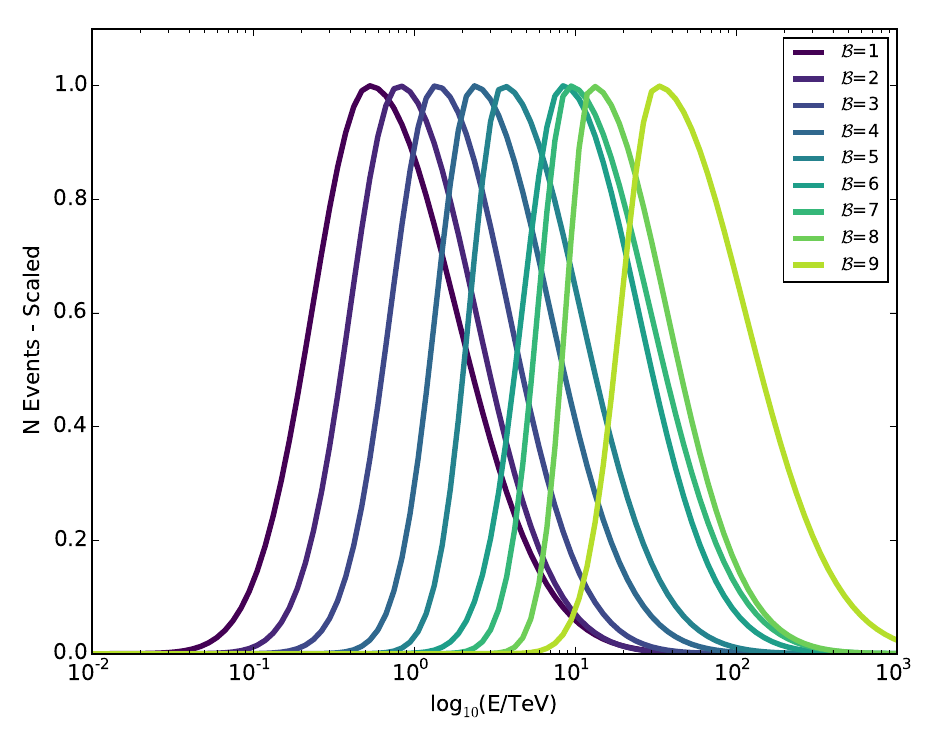
\includegraphics[scale=0.6]{figures/hawc/fhit_bins.png}
    }
    \caption{Simulated normalized energy distribution of each $f_\mathrm{hit}$ bin defined in \cref{tab:fhit_bins}. Monte Carlo simulation of gamma-rays with $E^-{2.63}$ spectral shape and simulated source at 20$^\circ$ declination. Figure from \cite{Abeysekara_2017}.}
    \label{fig:fhit_bins}
\end{figure}

\begin{table}
    \centering{
    \begin{tabular}{c?cc|c}
        \hline
        Bin &
        Lower Edge \% &
        Upper Edge \% &
        $\Theta_{68}$ ($^\circ$) \\
        \hline
        1       &
        6.7     &
        10.5    &
        1.05    \\

        2       &
        10.5    &
        16.2    &
        0.69    \\

        3       &
        16.2     &
        24.7    &
        0.50    \\

        4       &
        24.7     &
        35.6    &
        0.39    \\

        5       &
        35.6     &
        48.5    &
        0.30    \\

        6       &
        48.5     &
        61.8    &
        0.28    \\

        7       &
        61.8     &
        74.0    &
        0.22    \\

        8       &
        74.0     &
        84.0    &
        0.20    \\

        9       &
        84.0     &
        100    &
        0.17    \\

    \end{tabular}
    }
    \caption{Definitions of $f_\mathrm{hit}$ energy estimator bins. Bins are defined by the fraction of available PMTs that are triggered during an air shower event. The angular resolution, $\Theta_{68}$, is the bin containing 68\% of events \cite{Abeysekara_2017}.}
    \label{tab:fhit_bins}
\end{table}

The HAWC Observatory quantifies the primary particle energy of air showers using a metric known as $f_{\text{hit}}$.
This ratio compares the count of PMTs involved in the event reconstruction to the total number of functional PMTs at the time \cite{Abeysekara_2017}.
The main array consists of about 1200 PMTs, but the count may vary due to maintenance or other operational factors.

Events are stratified into several $f_{\text{hit}}$ bins.
Each bin corresponds to a specific range of angular resolutions, enabling a structured approach to event analysis based on the extent of the shower footprint, see \cref{tab:fhit_bins}.

The relationship between $f_{\text{hit}}$ and primary energy is complex; atmospheric attenuation can cause high-energy showers to present a smaller footprint, misrepresenting their energy in the $f_{\text{hit}}$ metric.
This effect is captured in simulations that chart the actual energy distribution across $f_{\text{hit}}$ categories \cite{wcd_Sensitivity}.
Such distributions vary with the declination of the source and the theoretical energy spectrum used in the model.
The $f_{\text{hit}}$ metric, while effective, has several limitations.
It is dependent on the zenith angle and the spectral characteristics presumed for the observed source.
The variable also reaches a saturation point around 10 TeV, after which the detector's ability to discriminate between higher energy levels diminishes \cite{Abeysekara_2017}.
Furthermore, the energy distribution for each $f_{\text{hit}}$ bin is notably broad, see \cref{fig:fhit_bins}.

In response to these limitations, HAWC has developed more intricate algorithms for energy estimation.
These algorithms incorporate the zenith angle and the distribution of charge around the shower core for a more accurate assessment of the primary particle's energy, particularly at energies surpassing 10 TeV \cite{wcd_Sensitivity}.
The following section describes the improvements made in energy estimation using a neutral network.

%$$$$$$$$$$$$$$$$$$$$$$$$$$$$$$$$$$$$$$$$$$$$$$$$$$$$$$$$$$$$$$$$$$$$$$$$$$$$$$$$$$$%
\subsection{Neural Network Energy Estimation}\label{sec:hawc_nn}
%$$$$$$$$$$$$$$$$$$$$$$$$$$$$$$$$$$$$$$$$$$$$$$$$$$$$$$$$$$$$$$$$$$$$$$$$$$$$$$$$$$$%

The energy estimation for photon events at the HAWC Observatory is refined through an artificial neural network (NN) algorithm.
This method, based on the Toolkit for Multivariate Analysis NN, adopts a multilayer-perceptron model with logistic activation functions across its layers.
The structure includes two hidden layers, the first with 15 nodes and the second with 14, designed to process input variables through a neural network optimized to estimate primary particle energies \cite{thesis_SamM}.

The NN is trained to minimize a specific error function that measures discrepancies between the NN's energy predictions and the actual energies from Monte Carlo simulations.
This minimization targets an error function that incorporates the relative importance of each event, weighting more an $E^{-2}$ power law spectrum.
This approach helps achieve a uniform error rate across energies ranging from 1 to 100 TeV.
The optimization process leverages the Broyden-Fletcher-Goldfarb-Shanno algorithm that calibrates the NN's 479 weights \cite{100TEV_Crab_HAWC}.

The spectral analysis employs a binned likelihood method, using a forward-folding technique to accommodate the energy estimate's bias and resolution \cite{100TEV_Crab_HAWC}.
This establishes a 2D binning scheme that categorizes events by both their $f_{\text{hit}}$ value and estimated energy.
The decision to use this scheme over a simple energy-based binning lies in the correlation between gamma/hadron separation parameters and the angular resolution with both the size and energy of the event.
The spectrum of interest is partitioned into nine $f_{\text{hit}}$ bins, each further divided into 12 energy bins, spanning from 0.316 TeV to 316 TeV, encompassing a total of 108 bins \cite{100TEV_Crab_HAWC}.
However, not all bins contribute to the final estimate.
Bins with low event populations or insufficient Monte Carlo simulation are excluded.
This approach focuses on the central 99\% of events by estimated energy within each $f_{\text{hit}}$ bin, effectively removing outliers \cite{100TEV_Crab_HAWC}.

\begin{figure}
    \centering{
        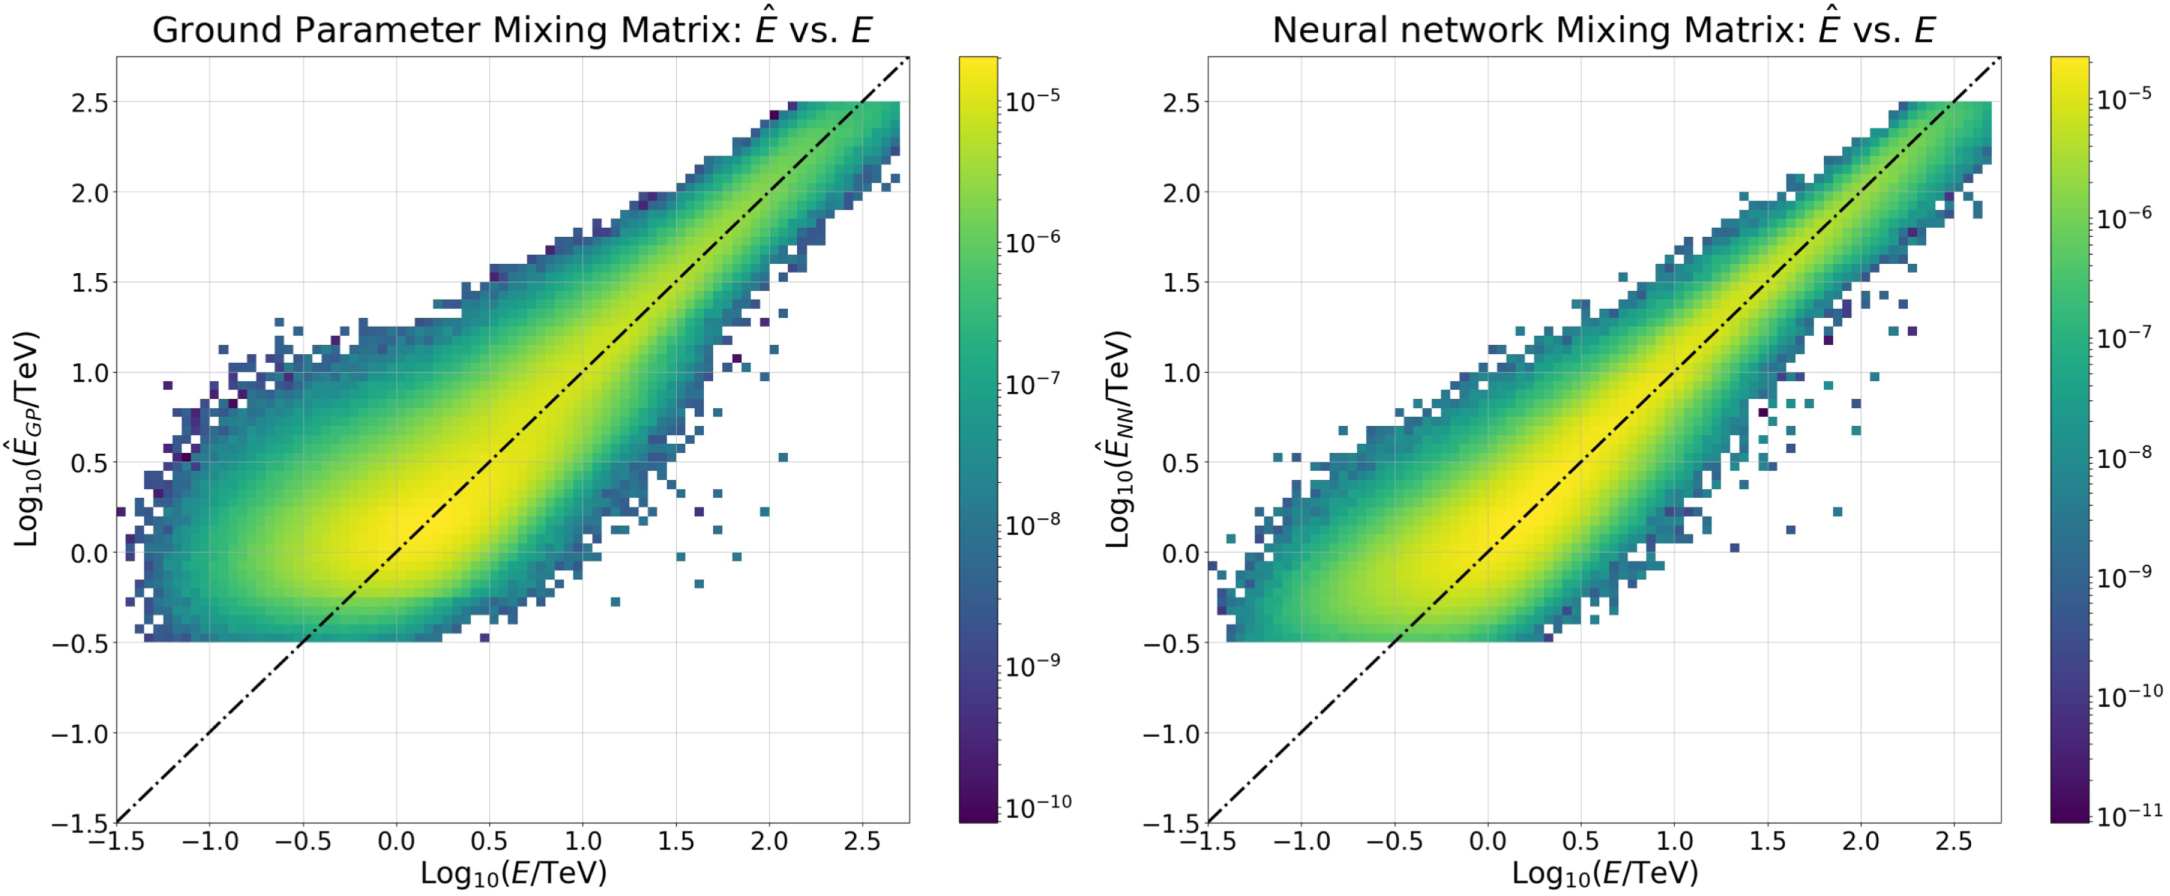
\includegraphics[clip, trim=9.1cm 0cm 0cm 0cm, scale=0.9]{figures/hawc/NN_performance.jpg}
    }
    \caption{Neural Network energy estimator performance compared to true energy. The dotted line is the identity line where the estimator and injection agree. Gamma/hadron separation cuts were applied with the energy estimation. Figure pulled from \cite{100TEV_Crab_HAWC}}
    \label{fig:NN_performance}
\end{figure}

Input variables for the NN are selected to capture key characteristics of the air shower: energy deposition, containment, and atmospheric attenuation.
The algorithm calculates energy deposition using the fraction of PMTs and tanks activated, alongside the logarithm of the normalization from the lateral distribution fit.
Containment is inferred from the distance between the shower core and the array's center, while atmospheric attenuation is evaluated using the reconstructed zenith angle and a detailed analysis of the shower's lateral charge distribution \cite{thesis_SamM,100TEV_Crab_HAWC}.
The performance on this NN is shown in \cref{fig:NN_performance}.

This refined NN energy estimation methodology is an integral component of HAWC's toolkit, enabling precise analysis of high-energy gamma-ray events.
It represents a significant advancement in the field by more accurately mapping observed shower characteristics to primary particle energies.

%$$$$$$$$$$$$$$$$$$$$$$$$$$$$$$$$$$$$$$$$$$$$$$$$$$$$$$$$$$$$$$$$$$$$$$$$$$$$$$$$$$$%
\subsection{G/H Discrimination}\label{hawc:gammaHadron}
%$$$$$$$$$$$$$$$$$$$$$$$$$$$$$$$$$$$$$$$$$$$$$$$$$$$$$$$$$$$$$$$$$$$$$$$$$$$$$$$$$$$%

\begin{figure}
    \centering{
        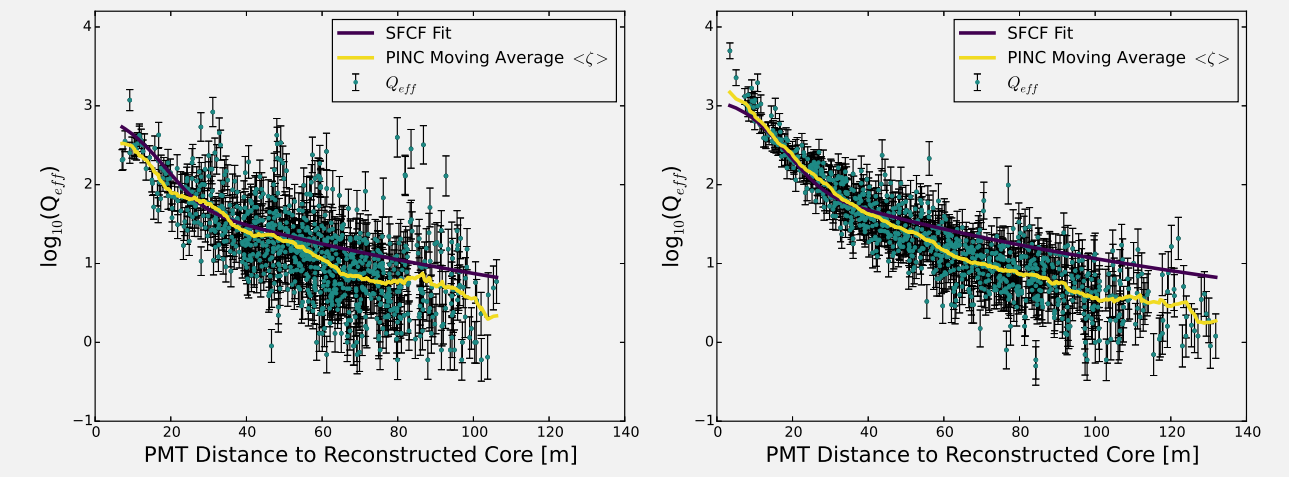
\includegraphics[scale=0.45]{figures/hawc/LDF_particles.png}
    }
    \caption{Lateral distribution functions (LDFs) for cosmic ray (left) and a photon candidate from the Crab Nebula (right). Cosmic ray LDF has clearly isolated hits far from the reconstructed shower core. Gamma-ray shower shows a more cuspy event \cite{Abeysekara_2017}.}
    \label{fig:ldf_particleshower}
\end{figure}

At the HAWC Observatory, distinguishing between air showers initiated by gamma rays and those by hadronic cosmic rays is fundamental for astrophysical data purity.
The separation process leverages differences in shower characteristics: electromagnetic showers from gamma rays typically display fewer muons and a smoother lateral distribution, whereas hadronic showers are more chaotic due to the abundance of muons and hadronic sub-showers.

Two primary parameters facilitate the identification of cosmic-ray events \cite{Abeysekara_2017}:

1) Compactness (C): This parameter evaluates the charge captured by PMTs, particularly focusing on the PMT with the highest effective charge beyond a 40-meter radius from the shower core.
Compactness is inversely proportional to this effective charge, as higher charges at extended distances from the core are indicative of hadronic showers.
It is mathematically expressed as:
\compactness
where $N_\mathrm{hit}$ is the number of PMTs hit and $CxPE_{40}$ is the effective charge measured outside a 40 m radius from the shower cores \cite{Abeysekara_2017}.

2) PINCness (P): PINCness quantifies the "clumpiness" of a shower using the charges recorded by PMTs and is short for Parameter for Identifying Nuclear Cosmic Rays.
It is computed from the logarithm of the effective charge, $Q_{\mathrm{eff},i}$, of each PMT hit, $i$, compared to an expected average for that annular region.
A higher PINCness suggests a less smooth distribution, typical of hadronic showers.
The formula is:
\pincness
where $\zeta_i = \log_{10}(Q_{\mathrm{eff},i})$.
The average, $\langle \zeta \rangle$ is the average over an annular region surrounding the shower core.
The errors, $\sigma_{\zeta_i}$, are computed and allocated from gamma-ray candidates close to the Crab.

These parameters are tested and modeled in simulations and with observational data near the Crab Nebula.
\Cref{fig:ldf_particleshower} illustrates the lateral distributions for representative cosmic-ray and photon candidate showers, and the Compactness and PINCness distributions \cite{Abeysekara_2017}.

The discrimination technique has remained consistent, but cut values have been reoptimized for the 2D bins based on $f_{\text{hit}}$ and NN estimated energy.
This refinement, referred to as Pass 5.F, enhances the selection of high-energy events.
Each bin ensures at least 50\% efficiency for gamma-ray detection, with efficiencies extending up to 99\% at the highest energy bins \cite{Abeysekara_2017,100TEV_Crab_HAWC}.

%$$$$$$$$$$$$$$$$$$$$$$$$$$$$$$$$$$$$$$$$$$$$$$$$$$$$$$$$$$$$$$$$$$$$$$$$$$$$$$$$$$$%
\section{Background Estimation: Direct Integration}\label{hawc:direc_int}
%$$$$$$$$$$$$$$$$$$$$$$$$$$$$$$$$$$$$$$$$$$$$$$$$$$$$$$$$$$$$$$$$$$$$$$$$$$$$$$$$$$$%

The ratio of cosmic rays to gamma rays can be as high as 10,000 to 1, depending on the energy.
At HAWC, we confront a significant challenge even after gamma/hadron cuts: our gamma-ray data is still inundated with cosmic-ray events.
To tackle this, we rely on the direct integration method developed by Milagro \cite{Milagro_crab}.
This method capitalizes on the cosmic rays' isotropic nature resulting from their deflection by interstellar magnetic fields.

The direct integration method estimates background events by integrating over a stable two-hour period of detector operation.
The expected number of background events at a particular sky coordinate ($\phi, \theta$) is determined by integrating the normalized detector's efficiency with the all-sky event rate:
\directInt
Here, $E(\text{ha}, \theta)$, represents the detector's efficiency, which varies with local coordinates (hour angle and declination).
$R(t)$ is the event rate as a function of time \cite{Milagro_crab}.

Our background estimation is expected to falter in high-energy ranges where cosmic-ray events are less frequent due to enhanced gamma/hadron discrimination. Sparsity in our background and data also arise at the limits of HAWC's sensitivity and during short-term analyses of transient events.
HAWC addresses these issues by using a pixel size of 0.5$^\circ$ in our direct integration to maintain robustness in our estimation \cite{Abeysekara_2017,wcd_Sensitivity}.
In constructing the background model, it's crucial to exclude areas of the sky with known gamma-ray sources.
Regions containing the Crab Nebula, Mrk 421, Mrk 501, and the Galactic Plane are masked to prevent their significant gamma-ray signals from biasing our background estimate \cite{Abeysekara_2017}.
